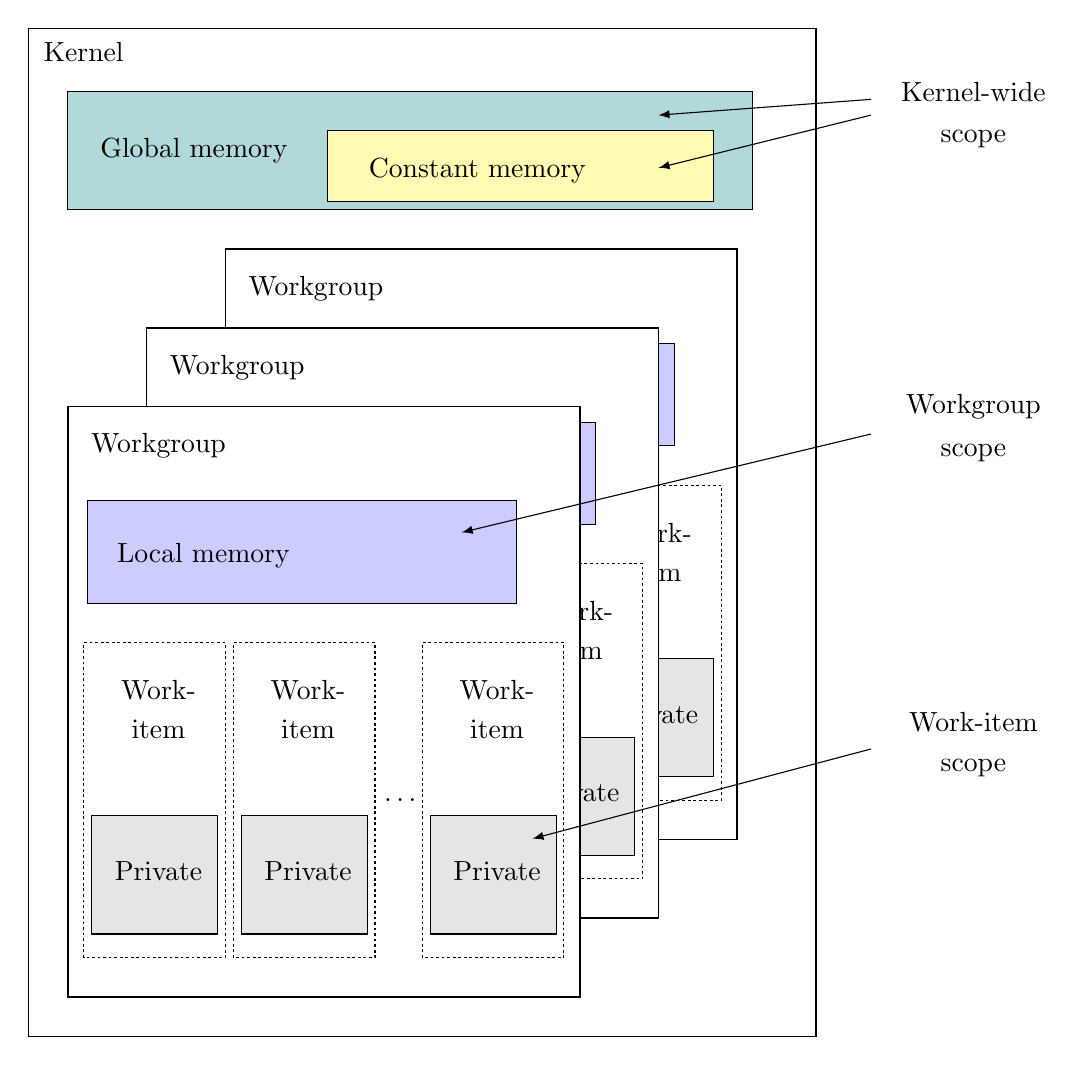
\begin{tikzpicture}[]
\draw[semithick] (0,0) rectangle (10,12.8);
\draw node at (0.7,12.5) {Kernel};
\foreach \x in {3,2,1}
{
  \draw[semithick,fill=white] (\x-0.5,\x-0.5) rectangle (\x+6,\x+7);
  \draw node at (\x+0.65,\x+6.5) {Workgroup};
  \draw[thin,fill=blue!20,fill opacity=40] (\x-0.25, \x+4.5) rectangle (\x+5.2, \x+5.8);
  \draw node [anchor=west] at(\x,\x+5.1) {Local memory};
  \foreach \y in {1, 2.90, 5.3}
  {
    \draw[thin,dashed, dash pattern = on 1pt off 1pt] (\x+\y-1.3, \x) rectangle (\x+\y+0.5, \x+4);
    \draw node at (\x+\y-0.35, \x+3.4) {Work-};
    \draw node at (\x+\y-0.35, \x+2.9) {item};
    \draw[thin,fill=gray!20,fill opacity=40] (\x+\y-1.20,\x + 0.3) rectangle (\x+\y+0.4,\x+1.8);
    \draw node at (\x+\y-0.35, \x+1.1) {Private};
  }
  \draw node at (\x+3.75, \x+2) {\ldots};
}

\draw[fill=blue!50!green!30] (0.5, 10.5) rectangle (9.2,12);
\draw node at (2.1, 11.25) {Global memory};

\draw[fill=yellow!30!] (3.8, 10.6) rectangle (8.7,11.5);
\draw node at (5.7, 11) {Constant memory};

\draw node at (12, 12) {Kernel-wide};
\draw node at (12, 11.4) {scope};
\draw[-latex] (10.7,11.9) -- (8,11.7);
\draw[-latex] (10.7,11.7) -- (8,11.03);

\draw node at (12, 8) {Workgroup};
\draw node at (12, 7.4) {scope};
\draw[-latex] (10.7,7.65) -- (5.5,6.4);

\draw node at (12, 4) {Work-item};
\draw node at (12, 3.4) {scope};
\draw[-latex] (10.7,3.65) -- (6.4,2.51);
\end{tikzpicture}